%!TeX ts-program = xelatex
%!TeX encoding = utf-8 Unicode
\documentclass[ieeetran]{article}
\usepackage{amsmath, amssymb}
\usepackage{graphicx}
\usepackage{wrapfig}

\title{Investment and Financial Management \\Lecture Notes}
\author{Efe Kamasoglu}

\begin{document}

\maketitle

\pagebreak

\section{Introduction \& Financial Analysis} % (fold)
\label{sec:introduction_&_financial_analysis}

\textbf{Corporate Finance:}
Identifying profitable investment projects + Determining optimal financing + Liquidity planning
=> \underline{Maximizing firm / enterprise value}

\subsection{Financial Analysis} % (fold)
\label{sub:}

\subsubsection{Firms' disclosure of financial information} % (fold)
\label{ssub:firms_disclosure_of_financial_information}

\textbf{Purpose of financial statements:}
\begin{enumerate}
  \item Firm-issued accounting reports with past performance info
\item Reliable source of info for shareholders and stakeholders\footnote{A \textbf{shareholder} \underline{is someone who owns stock in your company}, while a \textbf{stakeholder} \textit{(example: supplier, government)} \underline{focuses on the company's overall performance}, how it treats customers, partners, and employees, and how it impacts the community, among other things.} of the firm
  \item Filed with relevant listing authority
  \item Preperation under certain rules and standards (GAAP, IFRS)
\end{enumerate}

\textbf{\\Main types of financial statements:}
\begin{enumerate}
  \item Balance sheet / statement of financial position
  \item Income Statement 
  \item Statement of cash flows
  \item Statement of changes in shareholders' equity
\end{enumerate}
 
\subsubsection{Balance sheet / statement of financial position} % (fold)
\label{ssub:balance_sheet_statement_of_financial_position}

\textbf{Balance sheet / financial position:} snapshot of firm's financial position (assets, liabilities, shareholder's equity) at a given point in time

\textbf{\\Balance sheet equation:} Two sides must be equal: 
\underline{\textit{Assests = Liabilities + Shareholder's Equity}}

\begin{figure}[t]
  \centering
  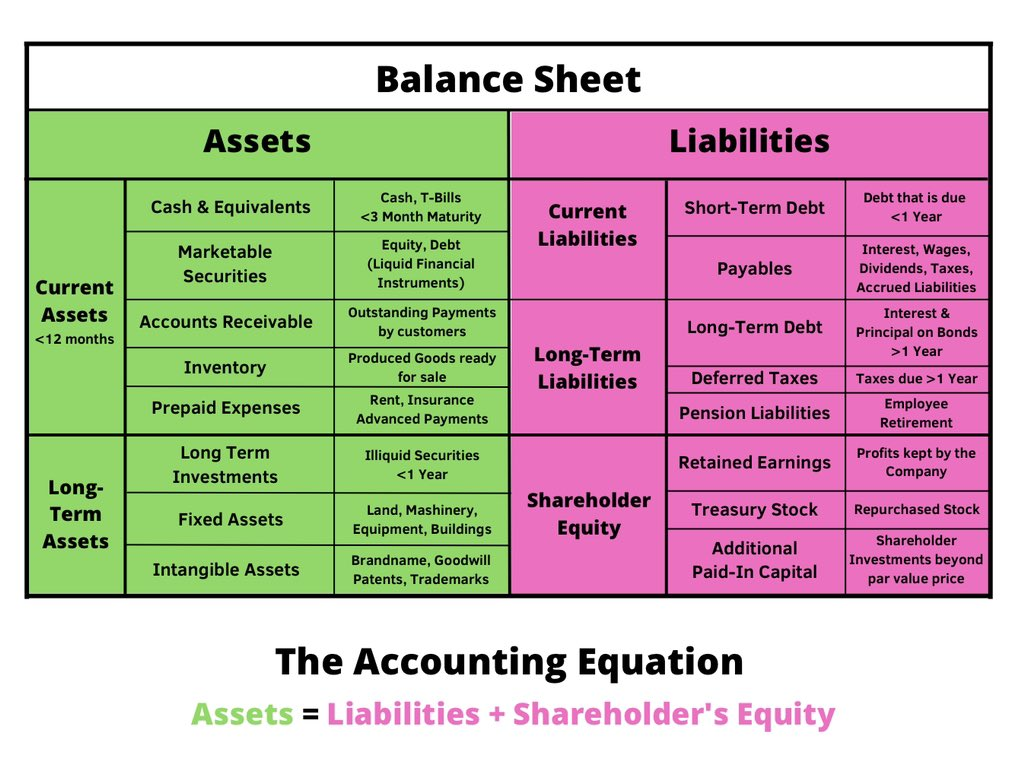
\includegraphics[width=0.58\linewidth]{balancesheet.jpg}
  \label{fig:balance_sheet_figure}
\end{figure}

\pagebreak

\begin{itemize}
  \item \textbf{Assets:} what the company owns
  \item \textbf{Liabilities:} what the company owes (debts, taxes etc.)
  \item \textbf{Shareholder's Equity:} difference between assets and liabilities
\end{itemize}

\begin{itemize}
  \item \textbf{Assets}
	\begin{itemize}
	  \item \textbf{Current Assests:} cash or expected to be turned into cash in the next year (not all operational!) \textit{(cash, marketable securities, accounts receivable, inventories)}
	  
	  \item \textbf{Non-current Assets (Fixed assets):} assets for long-term use (operational, more than one year) \textit{(net property, plant, equipment(PPE), goodwill and intangible assets)}
	\end{itemize}
   
\item \textbf{Liabilities}
	   \begin{itemize}
	     \item \textbf{Current Liabilities:} due to be paid within one year \textit{(accounts payable, short-term debt / notes payable, current maturities of non-current (long term) debt, taxes payable, wages payable)}
	     
	     \item \textbf{Net working capital (NWC):}
		     \large
		     \begin{equation*}
		     \boxed{NWC = Current \; Assets - Current \; Liabilities}
		     \end{equation*}
		     \normalsize
	     
	     \item \textbf{Non-current Liabilities:} to be paid beyond one year \textit{(long-term debt, capital leases, deferred taxes)}    
	   \end{itemize}

   \item \textbf{Shareholder's Equity: Book value vs. Market value}\footnote{\textbf{Book value} is the \underline{net value of a firm's assets} found on its balance sheet. \textbf{Market value} is the \underline{company's worth} based on the total value of its outstanding shares in the market, which is its market capitalization.}
	\begin{itemize}
	  \item \textbf{Book value of equity:}
		  \large
		  \begin{equation*}
		  \boxed{Book \; value \; of \; equity = 
		  Book \; value \; of \; assets - Book \; value \; of \; liabilities}
		  \end{equation*}
		  \normalsize
		  
		  \begin{itemize}
		    \item Could be negative
		    \item Many of the valuable assets may not be captured on the balance sheet	
		  \end{itemize}

	 \item \textbf{Market value of equity (= Market capitalization, market cap):}		 	 \large
		  \begin{equation*}
		  \boxed{Market \; value \; of \; equity = 
		  Market \; price \; per \; share * No. \; of \; shares \; outstanding}
		  \end{equation*}
		  \normalsize
		  \begin{itemize}
		    \item Cannot be negative
		    \item Often differs substantially from book value
		  \end{itemize}
	  
	  \item \textbf{Market-to-book (M/B) ratio (= Price-to-book (P/B) ratio):}
		 \large
		  \begin{equation*}
		  \boxed{M/B \; ratio = \frac{Market \; value \; of \; equity}{Book \; value \; of \; equity} 
		  }
		  \end{equation*}
		  \normalsize
		  \begin{itemize}
		    \item Successful firms have M/B ratio higher than 1
		    \item Value Stocks\footnote{A \textbf{value stock} is trading at levels that are \underline{perceived to be below its fundamentals}.}: Low M/B ratios
		    \item Growth stocks\footnote{A \textbf{growth stock} is any share in a company that is \underline{anticipated to grow} at a rate significantly above the average growth for the market \textit{(example: TSLA)}.}: High M/B ratios
		  \end{itemize}

  \end{itemize}
\item \textbf{Enterprise value (EV) (= Total enterprise value (TEV))}
	\begin{itemize}
	  \item Value of firm's underlying business operations / assets
	  \item Enterprise value $\neq$ Equity value 
		  \large
		  \begin{equation*}
		  \boxed{Enterprise \; value = 
		  Market \; value \; of \; equity + \underbrace{Debt - Cash}_\text{Net debt}}
		  \end{equation*}
		  \normalsize
	  \begin{itemize}
	  \item $Net \;  debt = Total \; debt - Cash \;  \& \; short\text{-}term \; investments$
	  \end{itemize}
subs
	\end{itemize}	
\end{itemize}


   

% subsubsection fdsfd (end)   
% subsubsection balance_sheet_statement_of_financial_position (end)
% subsubsection  (end)


% subsubsection firms_disclosure_of_financial_information (end)

% subsection  (end)


% section introduction_&_financial_analysis (end)

\subsubsection{Income statement} % (fold)
\label{ssub:subsubName}
\textbf{Income statement:} record of a firm's revenue, expense, and profit over a given period of time

\pagebreak

\begin{figure}[t]
  \centering
  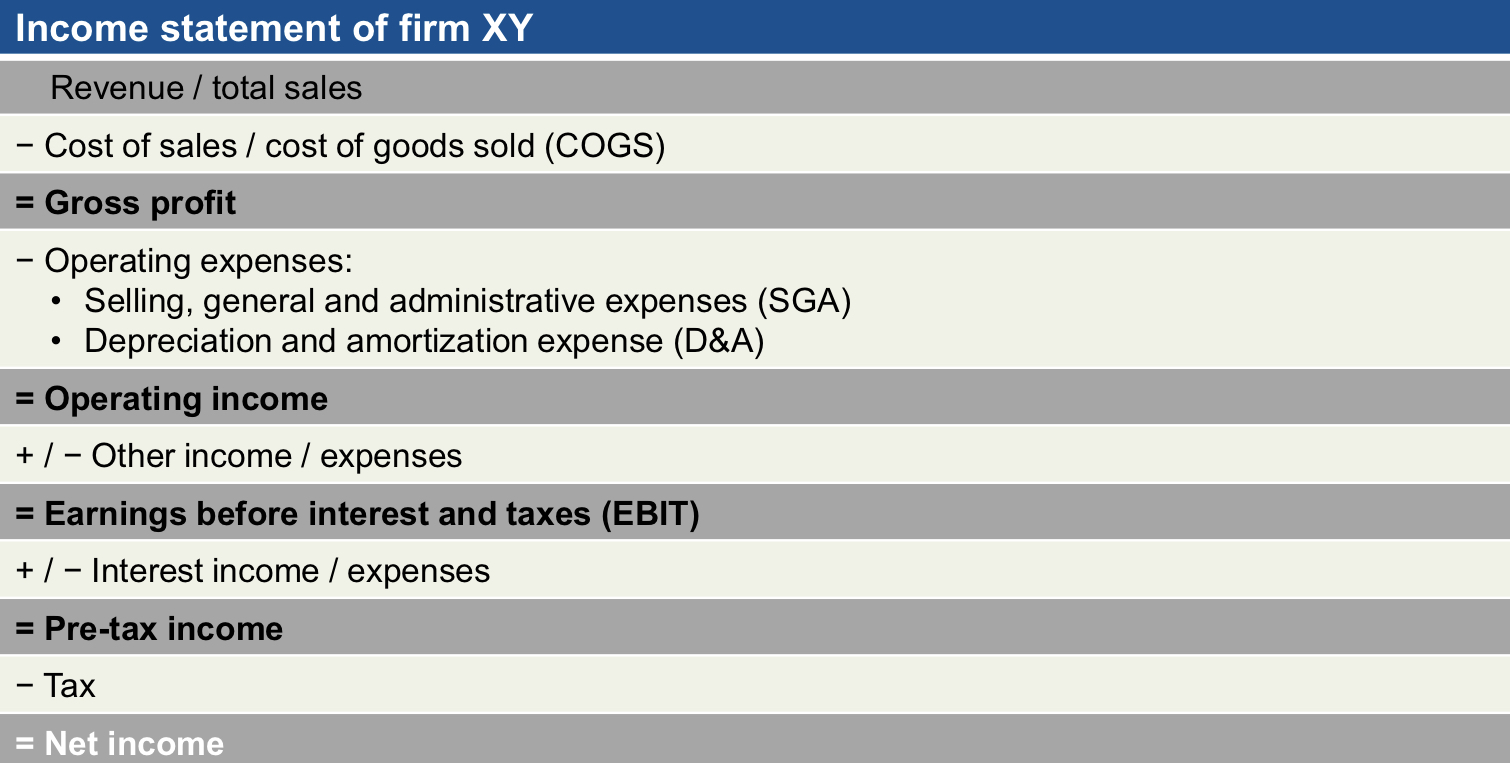
\includegraphics[width=1\linewidth]{incomestatement.jpg}
  \label{fig:income_statement_figure}
\end{figure}
\begin{itemize}
  \item \textbf{Net Income = Total earnings of the firm's equity holders}
	  \begin{itemize}
	    \item \textbf{Earnings per share (EPS):} how much money a company makes for each share of its stock
		   \large
		   \begin{equation*}
		   \boxed{EPS = \frac{Net \; income}{Shares \; outstanding}}
		   \end{equation*}
		   \normalsize

	   \item \textbf{Diluted earnings per share (Diluted EPS):}\footnote{\textbf{Dilution} occurs when a company \underline{issues new shares} that result in \underline{a decrease in existing stockholders' ownership percentage} of that company.} Future EPS could be diluted by in-the-money share (stock) options, convertible bonds or warrants. The diluted EPS takes these potential effects intp account.		   	

	  \end{itemize}

\end{itemize}

\subsubsection{Statement of cash flows} % (fold)
\label{ssub:statement_of_cash_flows}
\begin{itemize}
  \item Record of sources and uses of the firm's cash over a given period of time
	  \begin{itemize}
	    \item Sources of cash: activity that brings cash into firm \textit{(example: sales)}
	    \item Uses of cash: causes cash to leave firm \textit{(example: dividend payments\footnote{A \textbf{dividend} is the \underline{distribution of a company's earnings to its shareholders} and is determined by the company's board of directors.})}
	  \end{itemize}
	    \item Derived from firm's income statement and changes in balance sheet
	    \item Consists of:
		    \begin{itemize}
		      \item Cash flows from \textbf{operating}, \textbf{investing} and \textbf{financing} activities
		    \end{itemize}
\end{itemize}

\pagebreak
 
\subsubsection{Financial statement analysis} % (fold)
\label{ssub:}
\begin{itemize}
  \item \textbf{Financial ratios}
	  \begin{itemize}
	    \item Are used to:
		    \begin{itemize}
		      \item Compare firm with itself over time
		      \item Compare firm to other similar firms
		    \end{itemize}
	    \item Key financial ratios measure a firm's:
		    \begin{itemize}
		      \item Profitability
		      \item Liquidity
		      \item Working Capital
		      \item Interest Covarage
		      \item Leverage (Gearing)
		      \item Valuation
		      \item Operating Returns 
		    \end{itemize}
	  \end{itemize}

 \item \textbf{Profitability ratios}
	 \begin{itemize}
		 \item Measures of a firm's ability to generate profits as a percentage of the sales generated (margin ratios; margin = portion of sales that is a profit)
		\item Four levels of profitability ratios (resulting from income statement)
			\begin{enumerate}
			  \item 
			  \large
			  \begin{equation*}
			  \boxed{Gross \; margin = \frac{Gross \; profit}{Sales}}
			  \end{equation*}
			  \normalsize
			  
			  \item 
			  \large
			  \begin{equation*}
			  \boxed{Operating \; margin = \frac{Operating \; income}{Sales}}
			  \end{equation*}
			  \normalsize

			  \item 
			  \large
			  \begin{equation*}
			  \boxed{EBIT \; margin = \frac{EBIT}{Sales}}
			  \end{equation*}
			  \normalsize

			  \item 
			  \large
			  \begin{equation*}
			  \boxed{Net \; profit \; margin = \frac{Net \; income}{Sales}}
			  \end{equation*}
			  \normalsize
	  \end{enumerate}

	 \end{itemize}

\item \textbf{Liquidity ratios}
	\begin{itemize}
	  \item Measures of a firm's ability to meet short-term debt obligations
	  \item Help to assess firm's liquidity / financial solvency info of balance sheet / statement of financial position
	  \begin{enumerate}
	    	\item 
		\large
		\begin{equation*}
		\boxed{Current \; ratio = \frac{Current \; assets}{Current \; liabilities}}
		\end{equation*}
		\normalsize

	    	\item 
		\large
		\begin{equation*}
		\boxed{Quick \; ratio = \frac{Cash + Short\text{-}term \; investm. + Accounts \; receivables}{Current \; liabilities}}
		\end{equation*}
		\normalsize

	    	\item 
		\large
		\begin{equation*}
		\boxed{Cash \; ratio = \frac{Cash}{Current \; liabilities}}
		\end{equation*}
		\normalsize
	  \end{enumerate}
	\end{itemize}

\item \textbf{Interest coverage ratios}
	\begin{itemize}
	  \item Measures of a firm's ability to meet its interest payments by comparing its earnings with its interest expenses
	  \item Higher ratio = firm is earning much more than necessary to meet its obligations
	\end{itemize}
	  \begin{enumerate}
	    \item
	    \large
	    \begin{equation*}
	    \boxed{EBIT/Interest \; coverage = \frac{EBIT}{Interest \; expense}}
	    \end{equation*}
	    \normalsize

	    \item
	    \large
	    \begin{equation*}
		    \boxed{EBITDA/Interest \; coverage = \frac{\overbrace{EBITDA}^\text{EBIT + Depreciation/Amortization}}{Interest \; expense}}
	    \end{equation*}
	    \normalsize
	  \end{enumerate}

\item \textbf{Leverage / gearing ratios}
	\begin{itemize}
		\item Measures of a firm's reliance on debt as a source of financing
		\item Leverage ratios can be measured using book or market values!
          	\item Important and common ratios:
			\begin{enumerate}
	    			\item
	    			\large
	    			\begin{equation*}
					\boxed{Debt\text{-}equity \; ratio = \frac{Total \; debt}{Total \; equity}}
	   			\end{equation*}
	    			\normalsize 
				 
	    			\item
	    			\large
	    			\begin{equation*}
					\boxed{Debt\text{-}to\text{-}capital \; ratio = \frac{Total \; debt}{Total \; equity + Total \; debt}}
	   			\end{equation*}
	    			\normalsize

	    			\item
	    			\large
	    			\begin{equation*}
					\boxed{Debt\text{-}to\text{-}EV \; ratio = \frac{Net \; debt}{Market \; value + Net \; debt}}
	   			\end{equation*}
	    			\normalsize

	    			\item
	    			\large
	    			\begin{equation*}
					\boxed{Equity \; multiplier = \frac{Total \; assets}{Book \; value \; of \; equity}}
	   			\end{equation*}
	    			\normalsize
			\end{enumerate}
	\end{itemize}

\item \textbf{Valuation ratios}
	\begin{itemize}
	  \item Measures to help investors assess market value of a firm
	  \item These ratios are intended to make intra-industry comparisons of firm valuations.
	  \begin{enumerate}
	    \item
	    \large
	    \begin{equation*}
		    \boxed{
			\begin{aligned}
		    Price\text{-}to\text{-}earnings \; (P/E) \; ratio = \frac{Market \; capitalization}{Net \; income}\\
		    \\
		    = \frac{Share \; price}{Earnings \; per \; share}
			\end{aligned}
	    }
	    \end{equation*}
	    \normalsize

	    			\item
	    			\large
	    			\begin{equation*}
					\boxed{EV \; to \; EBIT = \frac{Market \; value \; of \; equity + Debt - Cash}{EBIT}}
	   			\end{equation*}
	    			\normalsize

	    			\item
	    			\large
	    			\begin{equation*}
					\boxed{EV \; to \; Sales = \frac{Market \; value \; of \; equity + Debt - Cash}{Sales}}
	   			\end{equation*}
	    			\normalsize				
	    
	  \end{enumerate}
	\end{itemize}

\item \textbf{Operating returns / investment returns}
	\begin{itemize}
	  \item Measures of a firm's returns on investment
       	  \item Compare its income to its investment using financial information from balance sheet / statement of financial position
		  \begin{enumerate}
		    \item 
		    \large
		    \begin{equation*}
		    \boxed{Return \; on \; equity \; (ROE)=\frac{Net \; income}{Book \; value \; of \; equity}}
		    \end{equation*}
		    \normalsize

		    \item 
		    \large
		    \begin{equation*}
		    \boxed{Return \; on \; assets \; (ROA)=\frac{Net \; income + Interest \; expense}{Total \; assets}}
		    \end{equation*}
		    \normalsize

		    \item 
		    \large
		    \begin{equation*}
		    \boxed{Return \; on \; invested \; capital \; (ROIC)=\frac{EBIT *  (1-Tax \; rate)}{Book \; value \; of \; equity + Net \; debt}}
		    \end{equation*}
		    \normalsize		    

		    \item 
		    \large
		    \begin{equation*}
		    \boxed{Asset \; turnover = \frac{Sales}{Total \; assets}}
		    \end{equation*}
		    \normalsize
		  \end{enumerate}
	\end{itemize}
\item \textbf{DuPont identity}
	\begin{itemize}
	  \item DuPont identity further decomposes return on equity (ROE) into theree components:
		  \begin{itemize}
		    \item Profitability (= Net profit margin)
	            \item Asset efficiency (= Asset turnover)
		    \item Leverage (= Equity multiplier)
			    \large
			    \begin{equation*}
				    \boxed{ROE = \underbrace{(\frac{Net \; income}{Sales})}_\text{Net profit margin} * \underbrace{(\frac{Sales}{Total \; assets})}_\text{Asset turnover} * \underbrace{(\frac{Total \; assets}{Book \; value \; of \; equity})}_\text{Equity multiplier}}
			    \end{equation*}
			    \normalsize
			    
		  \end{itemize}
	\end{itemize}
\end{itemize}
	
\subsection{Investment Analysis} % (fold)
\label{sub:investment_analysis}

\subsubsection{Net present value (NPV)} % (fold)
\label{ssub:net_present_value_nPV_}

\begin{itemize}
  \item \textbf{NPV (of a project or investment):} difference between present value of its benefits (cash inflow) and present value of its costs (cash outflow)

\large
\begin{equation*}
\boxed{
\begin{aligned}
NPV = PV(Benefits) - PV(Costs) =PV(All \; project \; cash \; flows)
\end{aligned}
}
\end{equation*}

\large
\begin{equation*}
\boxed{
\begin{aligned}
	NPV = \sum_{t=0}^{T} \frac{CF_t}{(1 + r)^t} 
\end{aligned}
}
\end{equation*}
\\
\normalsize
With:
\begin{itemize}
	\item NPV = Net present value, PV = Present Value, CF\textsubscript{t} = cash flow in period t, r = Appropriate discount rate
\end{itemize}

\item \textbf{NPV rule:}
	\begin{itemize}
	  \item \textbf{NPV decision rule:} When making an investment decision, take the alternative with the highest NPV.
     	  \item \textbf{Accepting or rejecting a project:}
		  \begin{itemize}
		    \item \underline{Accept, if positive NPV, expected profit} => equivalent to receiving its NPV cash today
		    \item \underline{Reject, if negative NPV, expected net loss} => would reduce the wealth of investors

		  \end{itemize}
	  \item \textbf{Alternative rules versus NPV rule:}
		  \begin{itemize}
		    \item Sometimes alternative investment rules give the same answer as the NPV rule, but at other times they disagree. \underline{If rules conflict, follow NPV decision rule.}
		    \item Equivalent rules: Economic value added (EVA), Annuity-rule
		  \end{itemize}
	\end{itemize}
\end{itemize}

\subsubsection{Internal rate of return (IRR)} % (fold)
\label{ssub:internal_rate_of_return_iRR_}
\begin{itemize}
  \item \textbf{IRR:} discount rate that makes NPV equal to zero (at which PV(Costs) = PV(Benefits))
	  \large
	  \begin{equation*}
	  \boxed{
	  \begin{aligned}
	  NPV = \sum_{t=0}^{N} \frac{CF_T}{(1+IRR)^t} = 0  
	  \end{aligned}
	  }
	  \end{equation*}
	  \\
	  \normalsize

	  With:
	  \begin{itemize}
	    \item NPV = Net present value, CF\textsubscript{t} = cash flow in period t,
		    IRR = Internal rate of return
	  \end{itemize}

\item \textbf{IRR rule:}
	\begin{itemize}
	  \item \textbf{IRR investment rule:}
		  \begin{itemize}
			  \item \underline{Take any investment, if its IRR exceeds cost of capital}\footnote{\textbf{Cost of capital} is the minimum rate of return or \underline{profit a company must earn before generating value} (e.g.\ undertaking a project, such as building new factory).}
			\item \underline{Turn any down investment, if its IRR is less than cost of capital}
		  \end{itemize}
	  \item \textbf{Application of IRR rule: IRR vs. NPV}
		  \begin{itemize}
			  \item IRR rule works for a stand-alone project if all of the project's \textbf{negative cash flows}\footnote{outgoing > incoming} precede \textbf{positive cash flows}\footnote{outgoing < incoming}. In other cases, \underline{IRR rule may disagree with NPV rule} thus be \underline{incorrect}!\\ 

			 \underline{\textit{Example:}}  \textit{If market conditions change over the years, project A can have multiple IRRs. Thus, IRR cannot be used. Instead, use NPV for comparison of projects.}
	
		  \end{itemize}
	  \item \textbf{Pitfalls of IRR rule:} Situations where IRR and NPV rules may conflict:
		\begin{enumerate}
		  \item Delayed investments
			  \item Multiple IRRs
				  \item Nonexistent IRR
		\end{enumerate}
		  \end{itemize}

\item \textbf{IRR vs. IRR rule:}
	\begin{itemize}
	  \item While IRR rule has shortcomings for making investment decisions, IRR itself remains useful.
	\item \textbf{But:}
		\begin{itemize}
		  \item IRR measures average return of investment => exact measure for average ROIC  of a project over its lifetime.
		  \item IRR can be used to check the sensitivity of NPV to any estimation error in the cost capital.
		\end{itemize}
	\end{itemize}
\item \textbf{Mutually exclusive projects:}
	\begin{itemize}
		\item When you must choose only one project among several possible projects, the choice is mutually exclusive\footnote{If two or more events are \textbf{mutually exclusive}, they \underline{cannot happen simultaneously}.}.
			\begin{itemize}
			  \item \underline{\textbf{NPV rule:}} Select the project with highest NPV.

			  \item \underline{\textbf{IRR rule:}} Selecting the project with the highest IRR may lead to mistakes.
			\end{itemize}
	\end{itemize}

\item \textbf{IRR rule and mutually exclusive investment with project ranking with different scales:}
	\begin{itemize}
	  \item If a project's size is doubled, its NPV will double. This is not the case with IRR. Thus, IRR rule cannot be used to compare projects of different scales.
	\end{itemize}

\item \textbf{Project ranking with timing of cash flows:}
	\begin{itemize}
	\item Problem with IRR: it can be affected by changing the timing of cash flows, even when the scale is the same.
	\item IRR is a return, but the dollar value of earning a given return depends on how long the return is earned.
	\item \underline{\textit{Example:}} \textit{A project with lower IRR can have a much higher NPV due to its higher growth rate.}
	\end{itemize}

\item \textbf{Project ranking with differences in risk:}
	\begin{itemize}
	  \item An IRR, that is attractive for a safe project, need not to be attractive for a riskier project.
	\item \underline{\textit{Example:}} \textit{IRR of a project is higher than those of the other investment opportunities, yet has the lowest NPV.}
	\item Higher cost of capital (e.g. due to size of the project) = Higher IRR
	\end{itemize}

\end{itemize}

\subsubsection{Other methods} % (fold)
\label{ssub:other_methods}

\begin{itemize}
\item \textbf{Payback method:}
	\begin{itemize}
	 \item \textbf{Payback period:} amount of time it takes to recover or pay back the initial investment (initial cash outflow).
\item \textbf{Payback rule:} \underline{Accept project}, if payback period is less than a pre-specified length of time. \underline{Otherwise reject}.

\item \textbf{Applicability of payback rule:} Payback rule is used by many companies due to its simplicity. Maybe, firms often care more about the liquidity drain of a project rather than its profitibility.

\item \textbf{Shortcomings of the payback rule:}
	\begin{itemize}
		\item Ignores the project's cost of capital and time value of money
			\footnote{\textbf{Time value of money} means that a sum of money is worth more now than the same sum of money in the future.\
			It can grow only \underline{through} \underline{investing so a delayed investment is a lost opportunity}.}
	\item Ignores cash flows after the payback period
	\item Relies on an ad hoc decision criterion
	\end{itemize} 
	\end{itemize}
 
\item \textbf{Probability index (PI):} PI can be used to identify the optimal combination of projects to undertake. Companies use it for evaluation of projects with different resource constraints.
	\large
	\begin{equation*}
	\boxed{
	\begin{aligned}
	Profitability \; index = \frac{Value \; created}{Resource \; consumed} = \frac{NPV}{Resource \; consumed}
	\end{aligned}
	}
	\end{equation*}
	\normalsize
\begin{itemize}
	\item \textbf{PI rule:} When choosing among projects competing for the same resource, pick the set of projects with the highest PIs that can still be undertaken given the limited resource.

\end{itemize}
\item \textbf{Shortcomings of PI:}
	\begin{itemize}
	  \item It does not take into account the size of the project, so it is not accurate in some cases.
	\item \underline{\textit{Example:}} \textit{A large project with lower profit margins may have a lower profitability index than a smaller project with higher profit margins.}
	\item Different combinations must be enumerated in order to find out NPV maximizing combination.
	\item With multiple resource constraints, PI can break down completely.
	\end{itemize}

\end{itemize}

\subsection{Capital Budgeting} % (fold)
\label{sub:capital_budgeting}
\textbf{Capital Budgeting:} A planning process used by a firm to determine if major projects or investments are worth the funding of cash capitalization structures (debt, equity or retained earnings)


% subsection capital_budgeting (end)

% subsubsection other_methods (end)
% subsubsection internal_rate_of_return_iRR_ (end)
% subsubsection net_present_value_nPV_ (end)

% subsection investment_analysis (end)


% subsubsection  (end)
% subsubsection statement_of_cash_flows (end)

% subsubsection subsubName (end)


\end{document}
